\documentclass[a4paper,12pt]{article}

\usepackage[utf8]{inputenc} % Kodowanie znaków
\usepackage{polski}         % Język polski
\usepackage{graphicx}       % Wstawianie obrazków
\usepackage{amsmath, amssymb} % Symbole matematyczne
\usepackage{hyperref}       % Linki w dokumencie
\usepackage{geometry}       % Ustawienia marginesów
\geometry{margin=2.5cm}     % Marginesy 2.5cm
\usepackage{indentfirst}    % Wcięcie w pierwszej linii
\usepackage{url}			 % Linkowanie w bibliografii

% Strona tytułowa
\title{\textbf{Metody rozwiązywania labiryntu}}
\author{Oskar Wiśniewski, 198058\\
 Mikołaj Wiszniewski 197925\\
 Franciszek Fabiński 197797 \\[0.5em]
Politechnika Gdańska, WETI}

\begin{document}

\maketitle

\section{Wstęp}
	Celem tego sprawozdania jest porównanie różnych, zaimplementowanych wcześniej metod rozwiązywania labiryntu: depth-first search, A* oraz Q-learning. W analizie skupiono się na takich aspektach jak skuteczność znajdowania rozwiązania, czas działania algorytmu oraz liczba odwiedzonych pól. Dodatkowo oceniono, jak poszczególne metody radzą sobie w labiryntach o różnym rodzaju zagęszczenia.

\section{Generowanie labiryntu}
	Wygenerowanie labiryntu opiera się na algorytmie opartym na algorytmie Kruskala ze strukturą zbiorów rozłącznych (disjoint set), który zapewnia utworzenie spójnej i acyklicznej siatki przejść – klasycznego labiryntu z jedną możliwą ścieżką pomiędzy dowolnymi dwoma punktami.
	\par Najpierw tworzona jest siatka ścian o rozmiarze \texttt{2*szerokość+1} na \texttt{2*wysokość+1}, w której wszystkie komórki są domyślnie oznaczone jako ściany. Następnie generowana jest lista możliwych ścian do usunięcia, tzn. są to wszystkie sąsiadujące komórki w siatce reprezentujące potencjalne przejścia między komórkami. Lista ta jest losowo tasowana, aby zapewnić różnorodność generowanych labiryntów.
	\par Dla każdej pary sąsiednich komórek sprawdzana jest przynależność do różnych zbiorów. Jeżeli tak – oznacza to, że usunięcie ściany między nimi nie utworzy cyklu. W takim przypadku ściana jest usuwana (komórki połączone są "korytarzem"), a zbiory są scalane.
	\par Dodatkowo, z prawdopodobieństwem \texttt{X}, usuwane są dodatkowe ściany boczne przylegające do tworzonego przejścia, co wprowadza rozgałęzienia i alternatywne ścieżki. Nadaje to labiryntowi bardziej złożony charakter.
	\par Na zakończenie, siatka jest obudowywana ścianą zewnętrzną oraz ustawiane są jedno wejście i wyjście w przeciwległych rogach labiryntu (lewy górny - wejście, prawy dolny - wyjście). Labirynt jest gotowy do wizualizacji oraz dalszego przetwarzania, np. przeszukiwania.

\section{Wyniki dla typowego labiryntu}

\subsection{Depth-first search}
	Ze względu na swoją prostotę, implementacja algorytmy DFS nie przysporzyła wielu problemów. Podczas testów dla większych labiryntów konieczna okazała się zmiana wersji rekurencyjnej na iteracyjną. Zauważono również silny wpływ kolejności sprawdzania wolnych pól na parametry wyjściowe programu, w szczególności kształt ścieżki. Wiąże się to z tym, że algorytm będzie wybierał stosunkowo częściej pola pod niższymi indeksami, ponieważ przeszukujemy "w głąb". Po testach najkorzystniejszą kolejnością okazała się $[(0, -1), (-1, 0), (0, 1), (1, 0)]$. Wynikowe ścieżki zwykle przebiegają w przybliżeniu wzdłuż górnej i prawej krawędzi labiryntu, co pokazano poniżej.
\begin{center}
    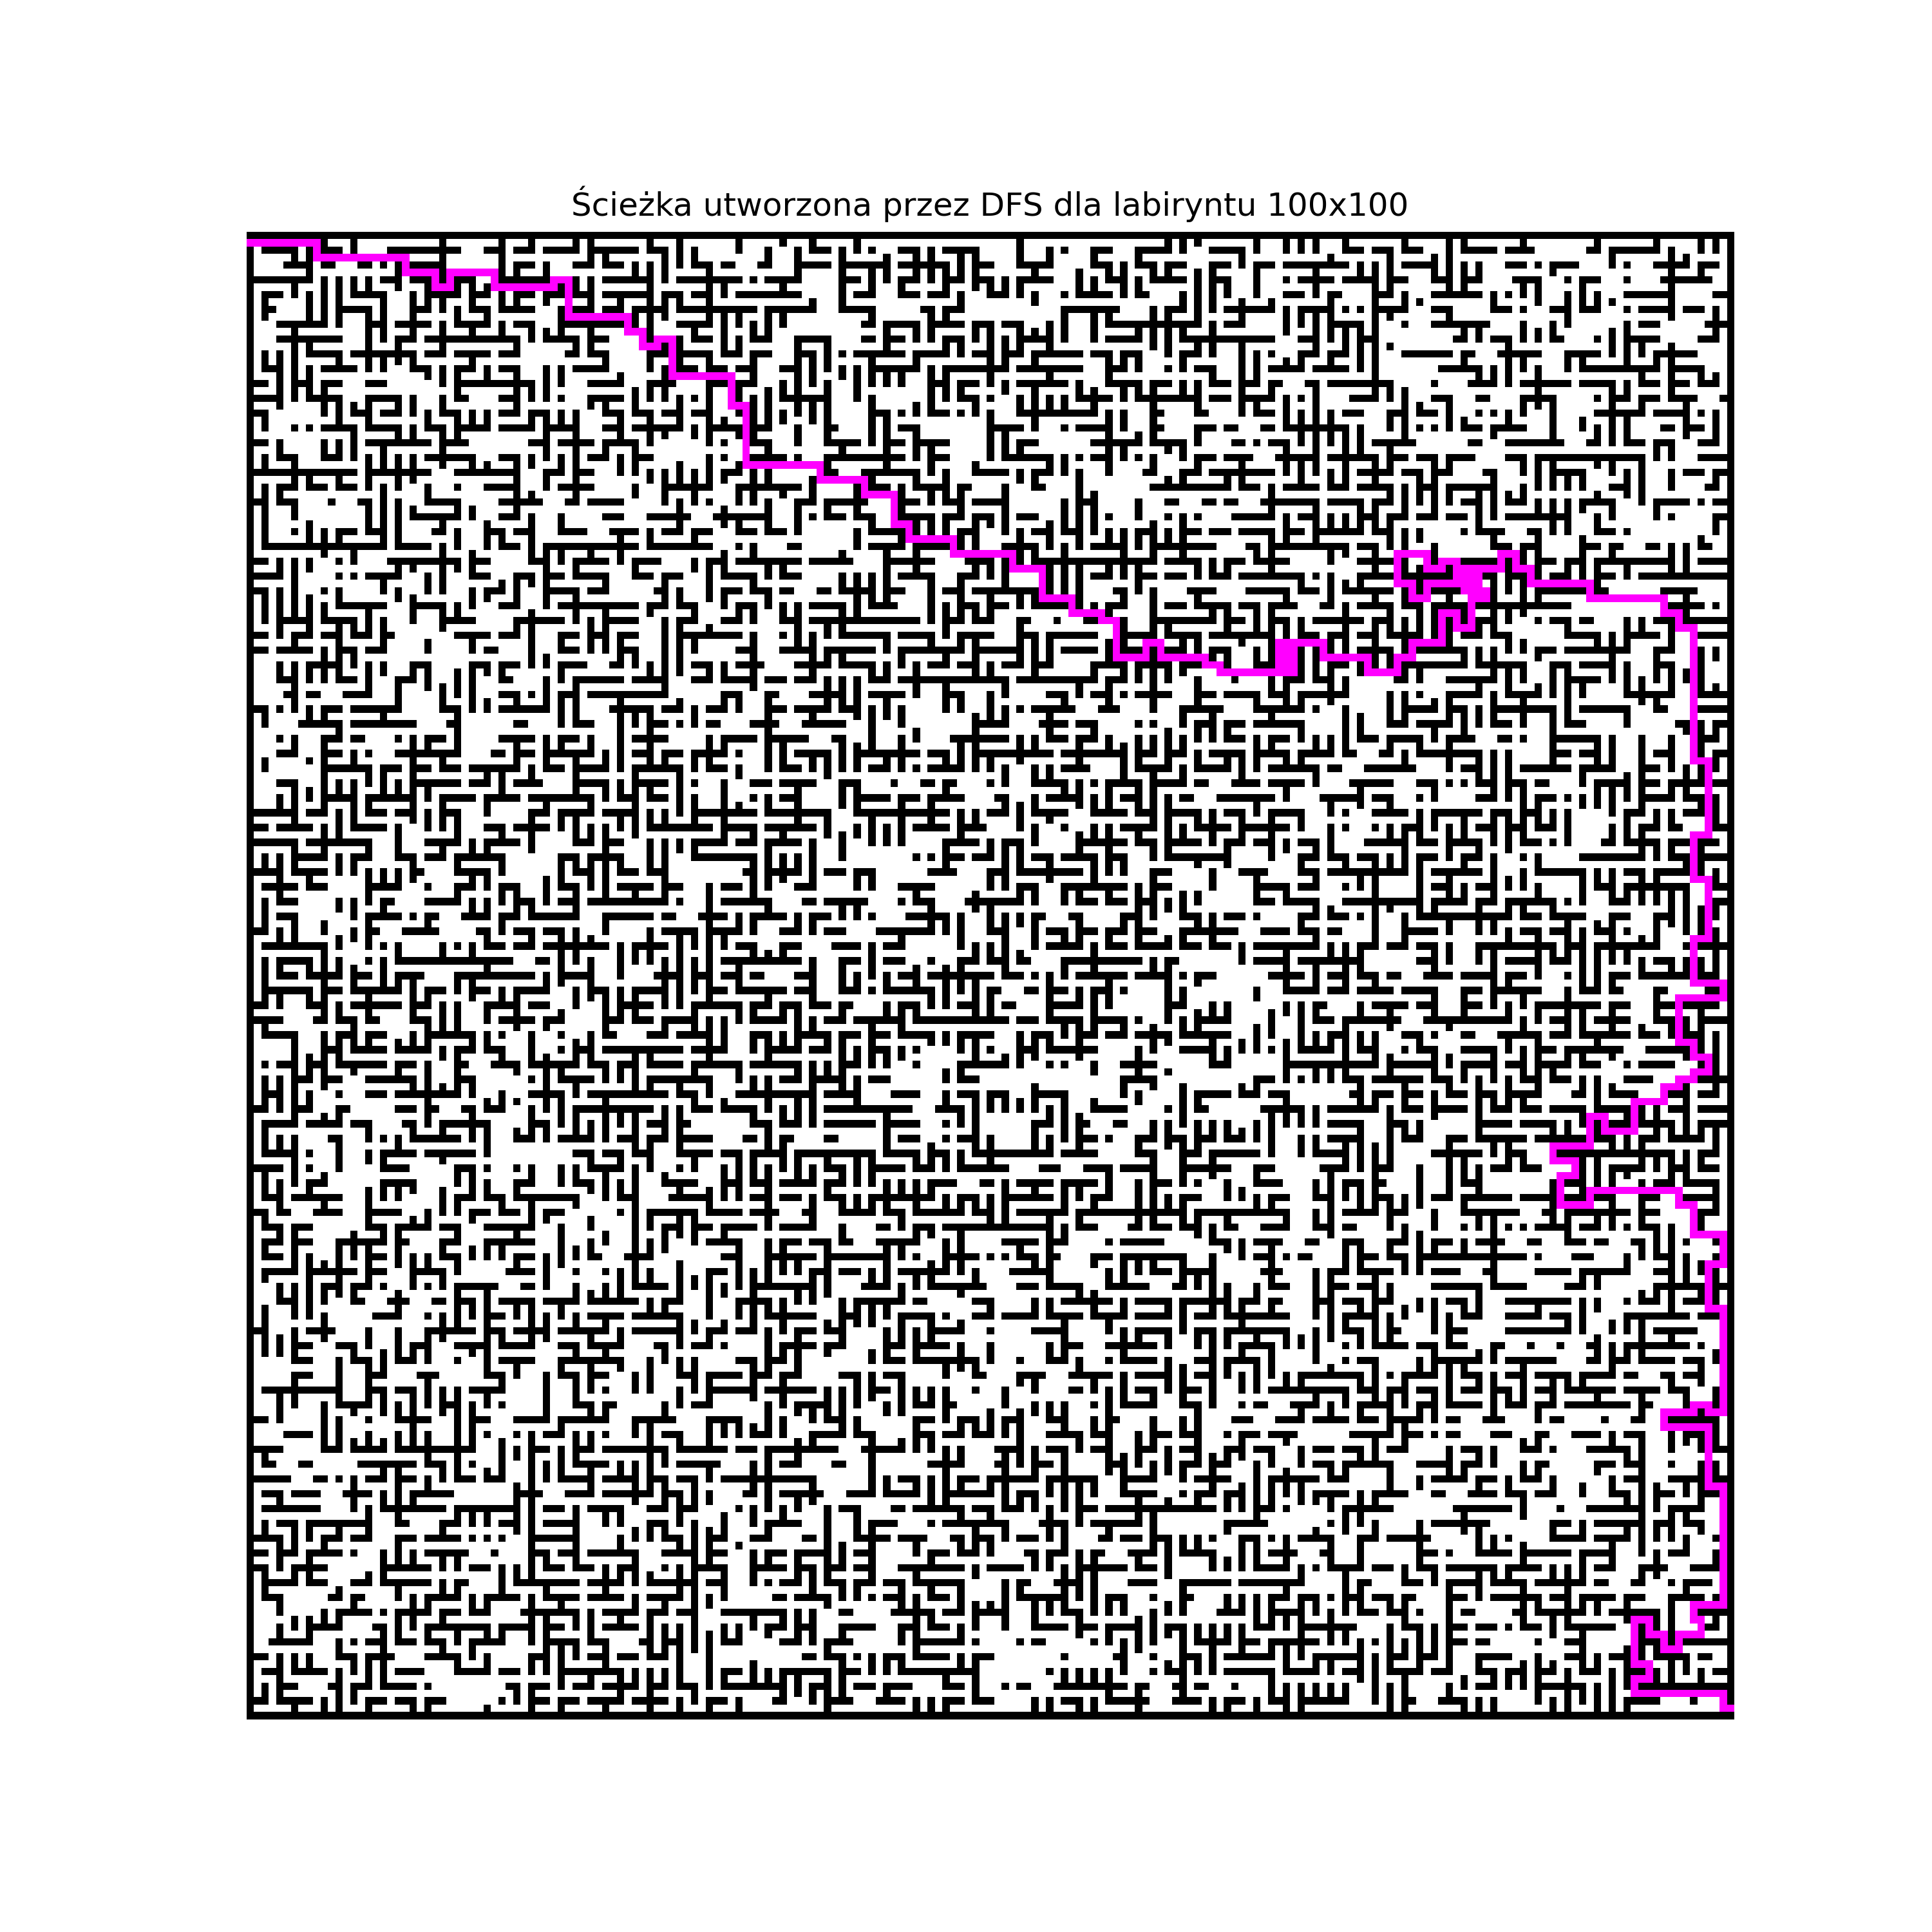
\includegraphics[width=0.7\textwidth]{../images/DFS_path.png}
\end{center}

\subsection{A*}
	W algorytmie A* wykorzystano heurystykę Manhattan, która polega na obliczaniu odległości pomiędzy dwoma punktami jako sumy wartości bezwzględnych różnic ich współrzędnych poziomych i pionowych. Jest to podejście szczególnie dobrze dopasowane do środowisk reprezentowanych w postaci siatki, gdzie możliwy jest wyłącznie ruch w czterech kierunkach: góra, dół, lewo i prawo. Z tego powodu był to pierwszy wybór przy implementacji. Z tego powodu wynikowe ścieżki zwykle biegną w przybliżeniu wzdłuż przekątnej od punktu wejściowego do wyjściowego, co pokazano poniżej.
\begin{center}
    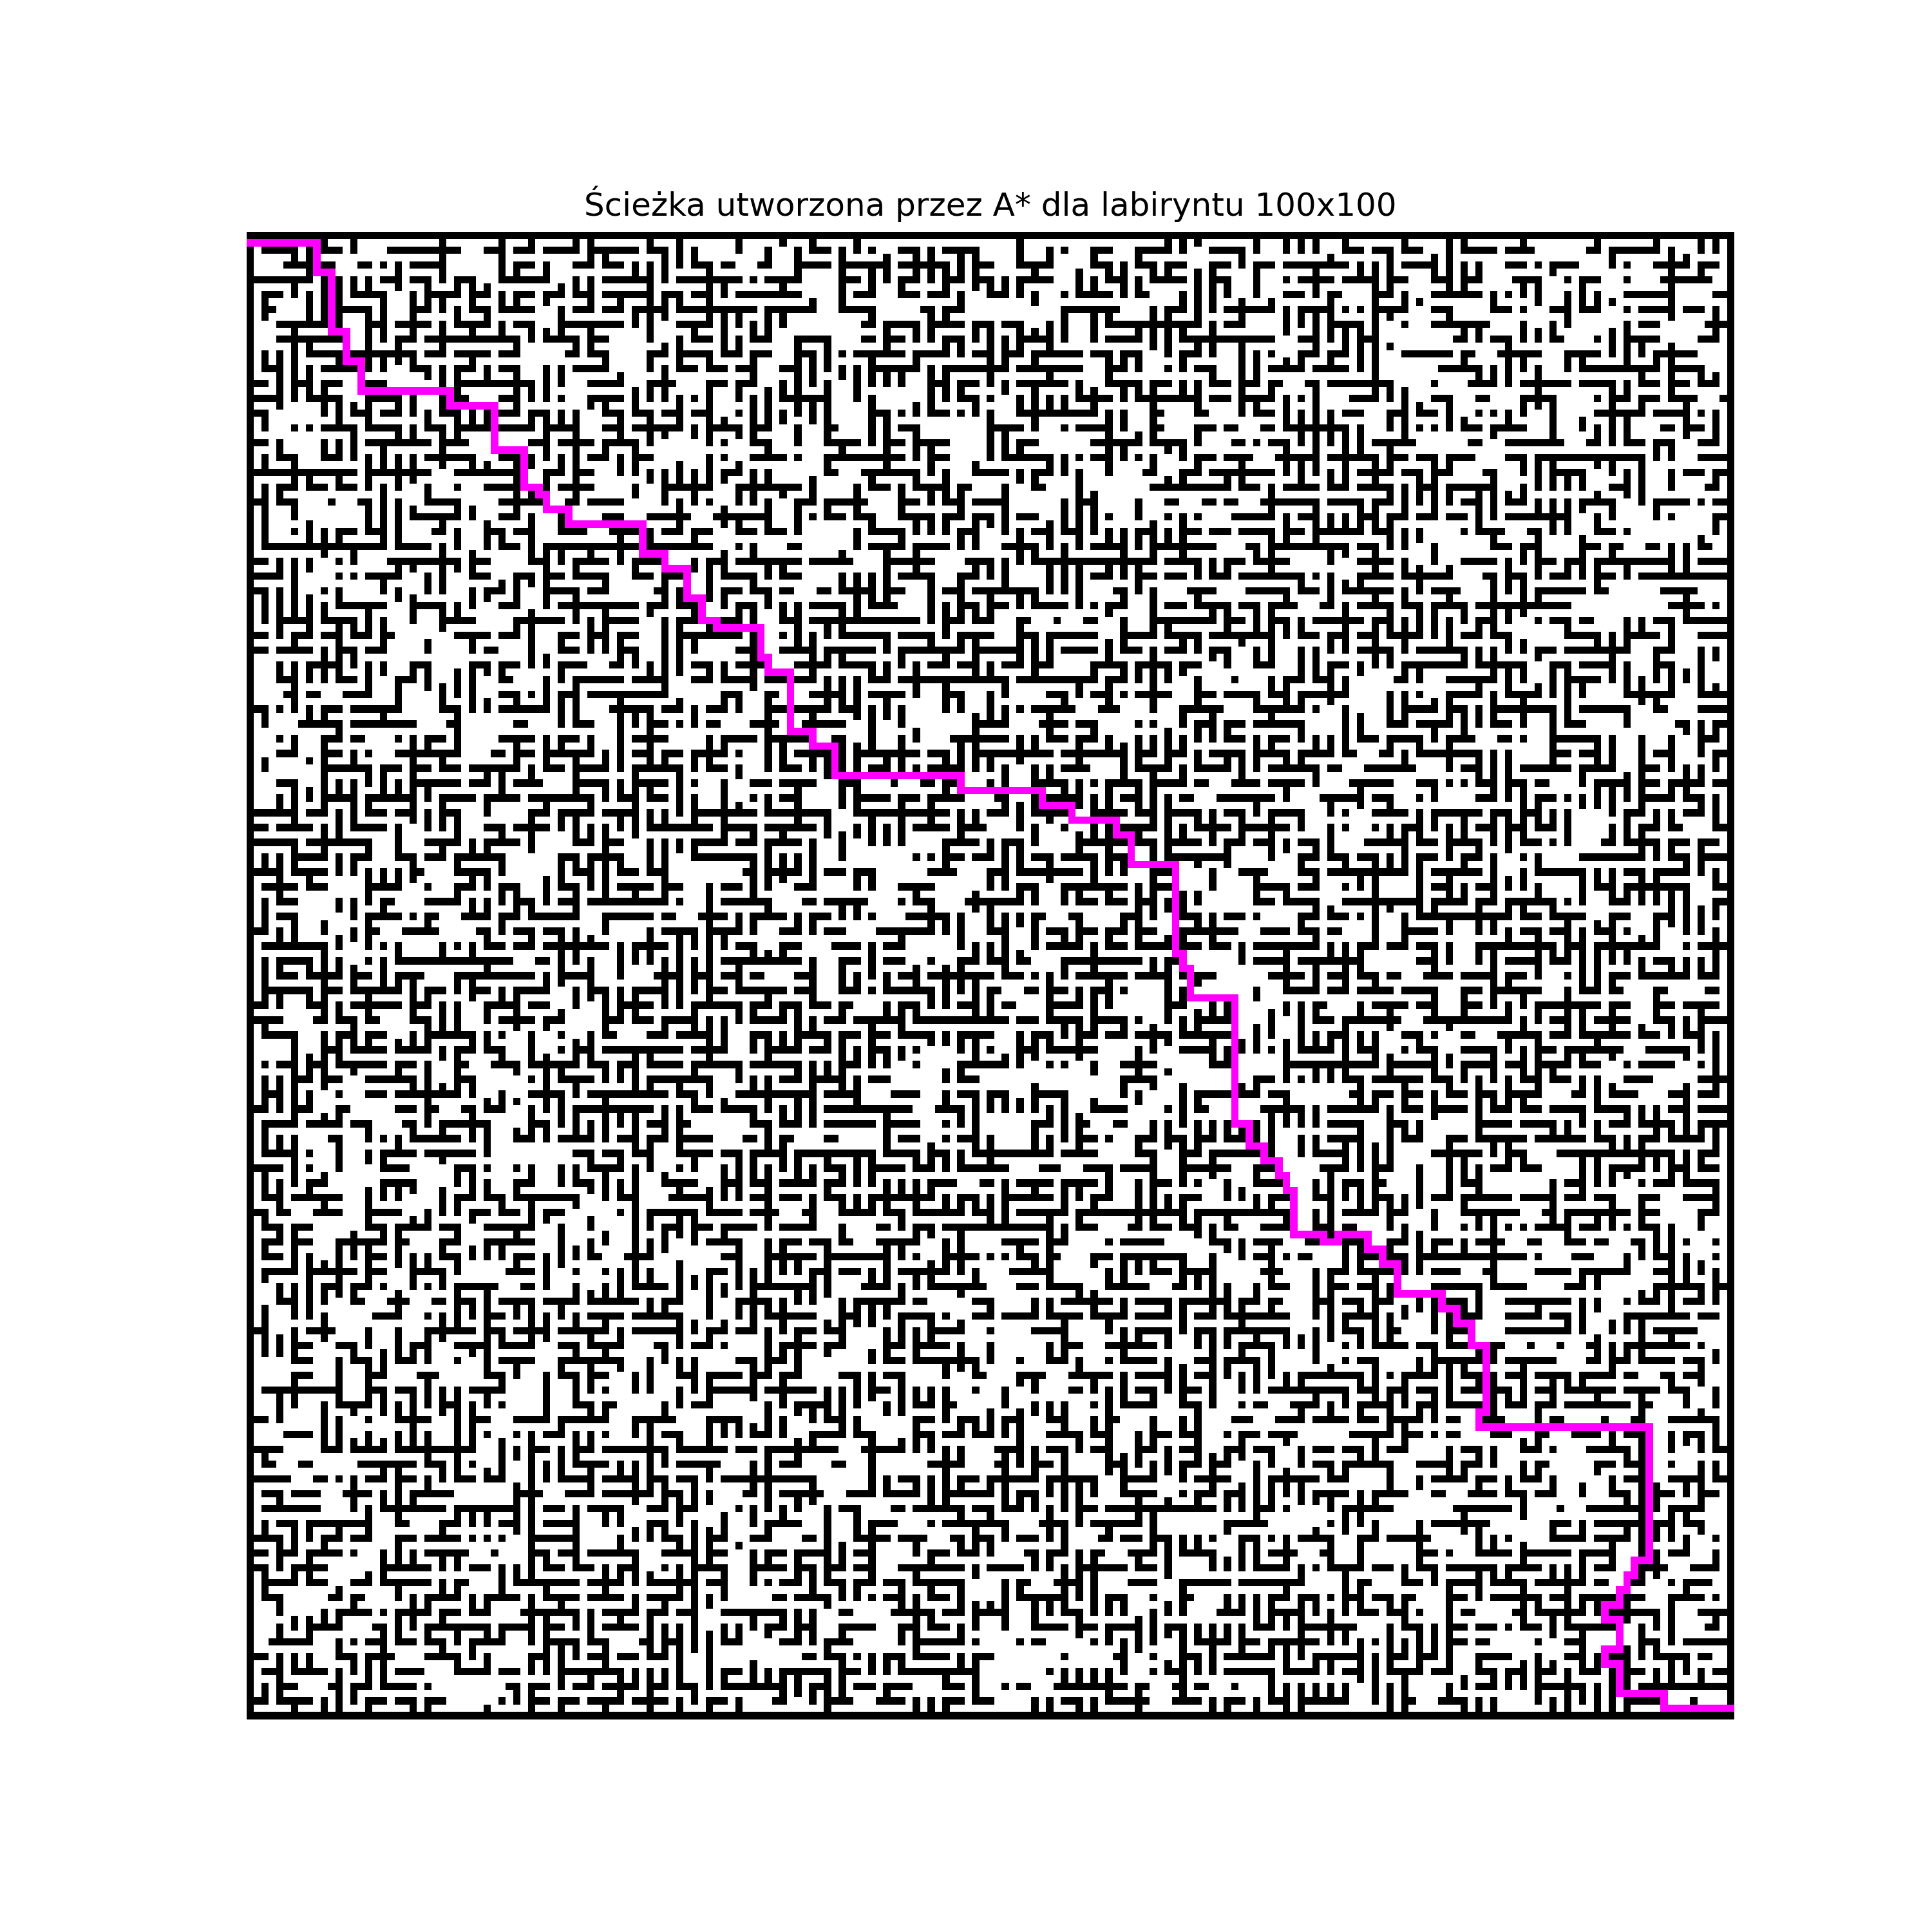
\includegraphics[width=0.7\textwidth]{../images/A*_path.png}
\end{center}

\subsection{Q-learning}
% opis problemow, zalozen, parametrow i wygenerowac sciezke 
    \subsubsection{Parametry}
    Dostępne parametry:
    \begin{itemize}
        \item alpha - learning rate
        \item beta - discount factor, faworyzacja późniejszych nagród
        \item epsilon - szansa na eksplorację (losowa akcja)
        \item episodes - liczba iteracji
    \end{itemize}
    Dobór parametrów ma duży wpływ na wydajność algorytmu.

    \subsubsection*{Episodes}
    Liczbę epizodów stosunkowo łatwo wybrać, wystarczy kilka razy włączyć program, żeby zobaczyć jaka jest ich najlepsza liczba w stosunku do czasu wykonania.
    W przypadku naszego algorytmu było to \textbf{5000}.
    Dla epizodów w liczbie 500-3000 wyniki nie były zadowalające, a epizody 5000-10000 miały pomijalnie mały wpływ na wydajność wytrenowanego modelu, a kosztowały czas.
    
    \subsubsection*{Beta}
    Ze względu na dużą liczbę epizodów oraz fakt, że dotarcie do wyjścia labiryntu oferowało dużą nagrodę, należało dobrać taki discount factor, żeeby model faworyzował późniejsze nagrody.
    W implementacji wynosi \textbf{0.99}.

    \subsubsection*{Alpha oraz epsilon}
    Zarówno $\epsilon$ jak i $\alpha$ w początkowych etapach był stałe, jednak po kilku próbach można było zauważyć, że nie jest to optymalne rozwiązanie.

    Lepszym sposobem jest zwiększenie tempa nauki oraz eksploracji w początkowych fazach trenowania, ponieważ model nie jest w stanie osiągnąć celu i heurystyka pomaga wypełniać qtable dobrymi wartościami.
    
    Ostatecznie w każdym epizodzie:
    \begin{itemize}
        \item \texttt{$\epsilon$ = max($\epsilon_{min}$, $\epsilon * \epsilon_{decay}$)}
        \item \texttt{$\alpha$ = max($\alpha_{min}$, $\frac{\alpha_0}{1 + ep * \alpha_{decay}}$)}
    \end{itemize}
    
    gdzie:
    \begin{itemize}
        \item $\epsilon_{min} = 0.1$
        \item $\epsilon_{decay} = \sqrt[ep]{\epsilon_{min}}$\
        \item $\alpha_{min} = 0.01$
        \item $\alpha_0 = 0.5$
        \item $\alpha_{decay} = 0.001$
        \item $ep$ to numer aktualnego epizodu
    \end{itemize}

    Takie wartości uznaliśmy za optymalne przy postawionym problemie i skutecznie maksymalizują one stosunek wydajności wytrenowanego modelu do czasu nauki.

    \subsubsection{Nagrody}
    Kolejnym problemem napotkanym przy implementowaniu  algorytmu był dobór nagród.
    Nagroda musi być na tyle duża, żeby miała wpływ na wybraną ścieżkę, jednak na tyle mała, że nie zamknie się on na pierwsze znalezione rozwiązanie.
    
    Dużym usprawnieniem działania było dodanie heurystyki opartej o manhattan distance agenta od celu.
    W każdej iteracji agent dostaje informację czy jest bliżej (\texttt{reward = 1}), bądź dalej (\texttt{reward = -1}).
    W przypadku dojścia do celu nagroda jest równoważna z długością ścieżki znalezioną przez algorytm A* (założenie, że jest to optymalna ścieżka).

    \subsubsection{Rezultat}
    
\begin{center}
    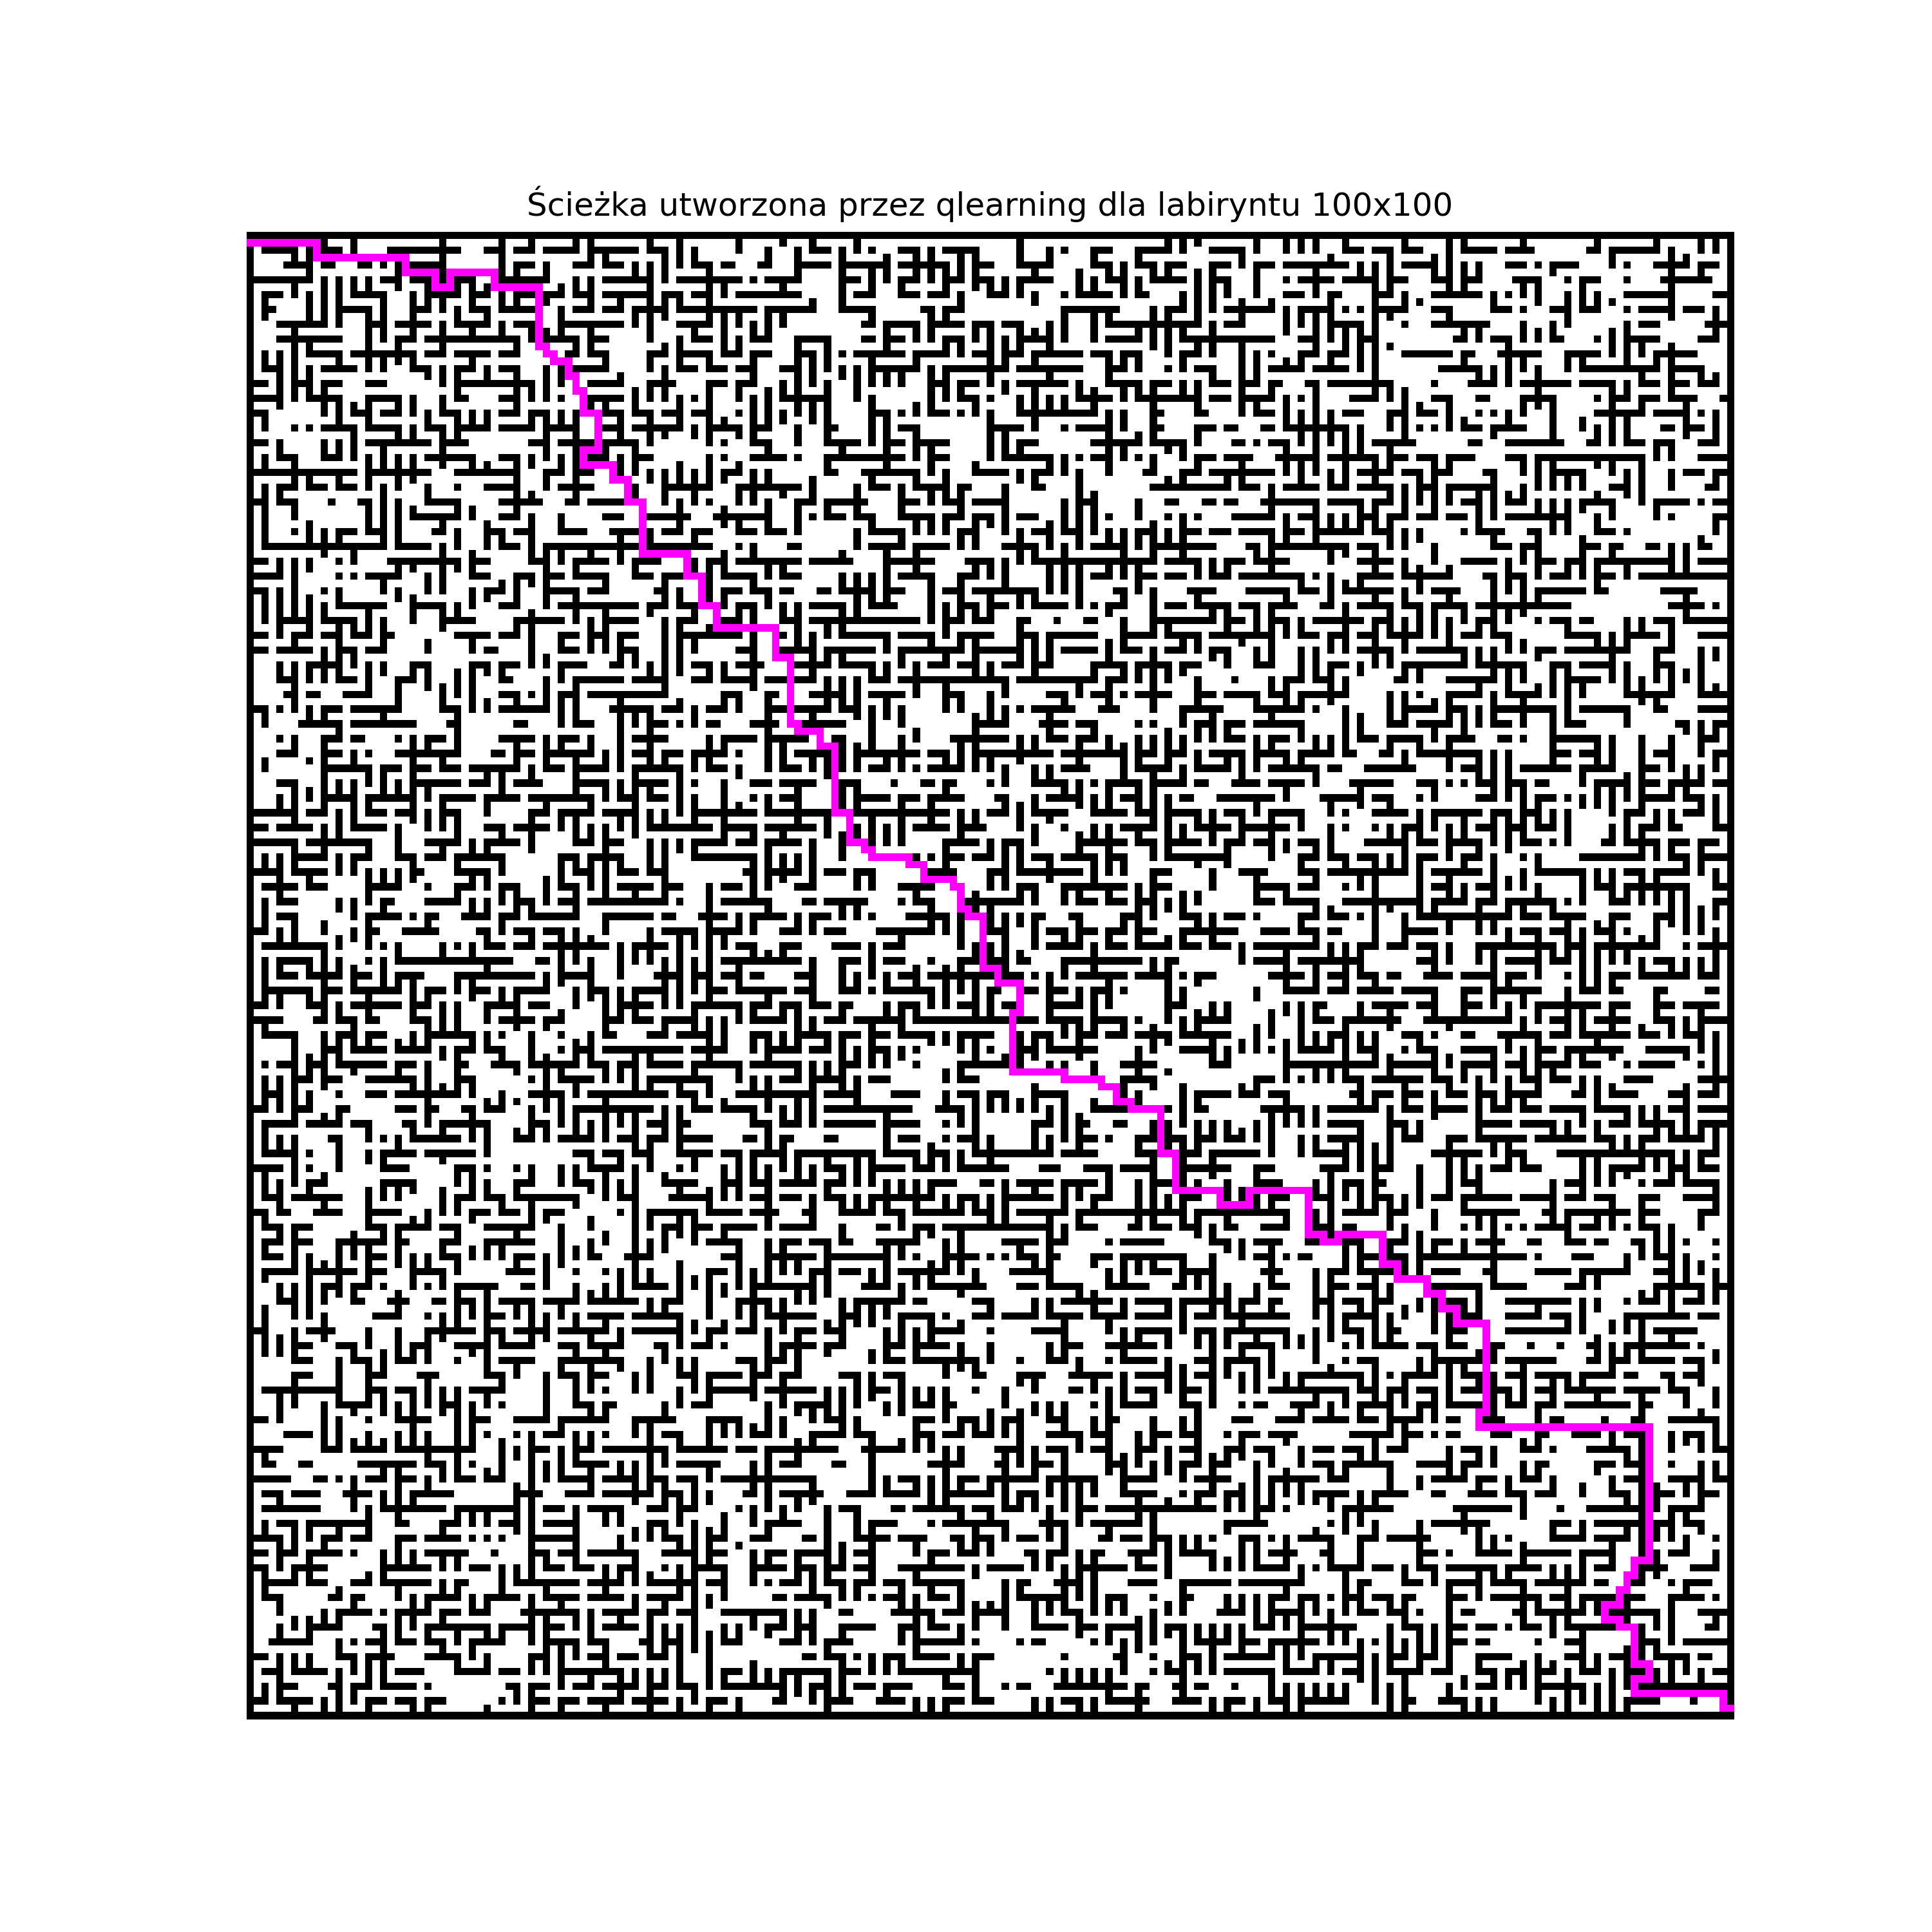
\includegraphics[width = 0.7\textwidth]{../images/qlearning_path.png}
\end{center}

    Powyższa grafika pokazuje ścieżkę znalezioną przez wyuczonego agenta. Widać, że ze względu na użycie tej samej heurystyki trasa ta przypomina rozwiązanie algorytmu A*.
    Trasa biegnie po przekątnej, więc nie ma dużego pola do optymalizacji i nauczony model można uznać za poprawny.
    
    \newpage
    \subsection{Porównanie}
	Poniżej pokazane jest porównanie wspomnianych do tej pory algorytmów A*, DFS oraz Q-Learning:
    \begin{center}
        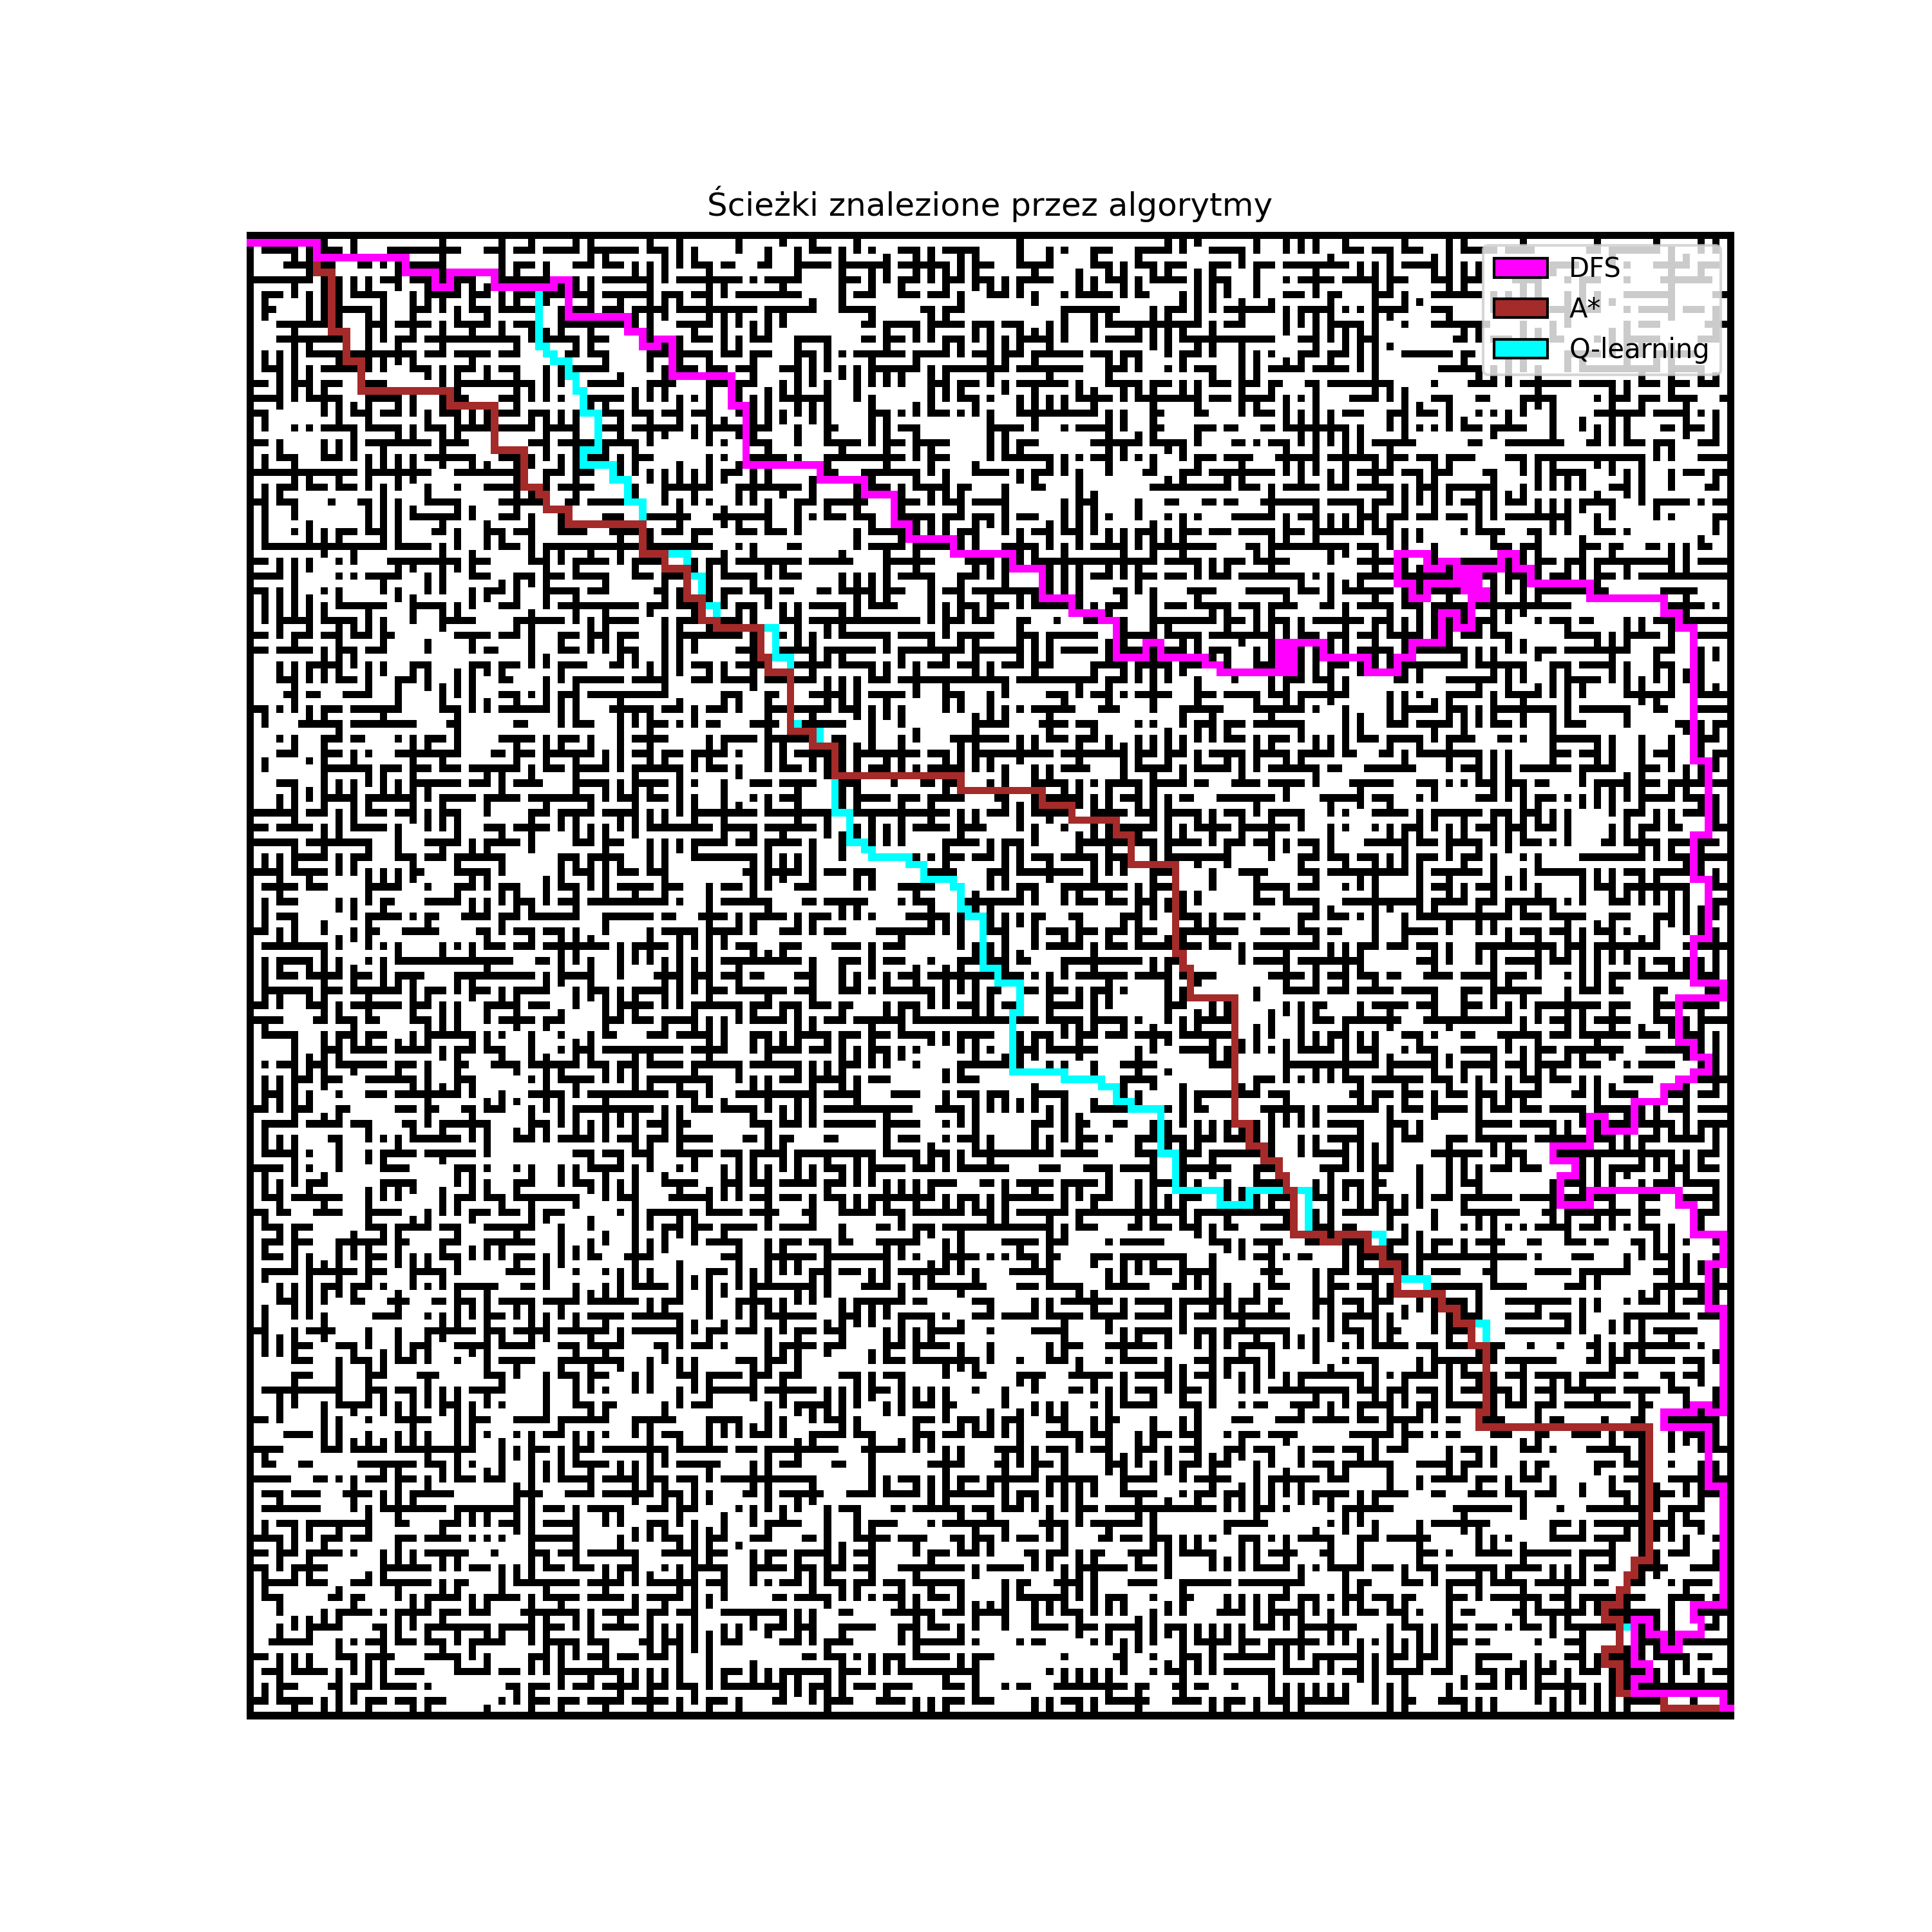
\includegraphics[width=0.7\textwidth]{../images/qlearning-vs-others.png}    
    \end{center}

    Oraz tabela przedstawiająca ich wydajność:
    \begin{table}[h!]
\centering
\begin{tabular}{|l|c|c|c|}
\hline
\textbf{Algorytm} & \textbf{Długość ścieżki} & \textbf{Czas wykonania (s)} & \textbf{Odwiedzone węzły} \\
\hline
DFS        & 637  & 0.0045  & 857    \\
A*         & 419  & 0.0332  & 11918  \\
Q-Learning & 433  & 0.0013  & 432    \\
\hline
\end{tabular}
\end{table}

    Trening modelu zajął \texttt{22.55} sekundy, a liczba odwiedzonych węzłów przez cały proces to \texttt{109,992,906}.

    \pagebreak
\section{Nauczanie heurystyki}

\subsection{Cechy}

  Na potrzeby stworzenia wyzwania, w którym nauczona heurystyka mogłaby się
  wykazać, zdecydowaliśmy się na stworzenie labiryntu o zwiększonym zagęszczeniu
  ścian w pobliżu środka i nadanie poszczególnym polom wag równym liczbie
  otaczających je ścian.

  Przy nauczaniu heurystyki model zwracał uwagę na następujące cechy:
  \begin{itemize}
    \item Odległość do celu (Manhattan distance) 
    \item Kierunek ruchu
    \item Wagi pól otaczających
  \end{itemize}

\subsection{Nauka}

  \subsubsection{Dane treningowe}
  Za dane treningowe posłużyły nam qtable z algorytmu Q-learning.
  Pierwsze przejście algorytmu zostało wykonane klasycznie - start znajdował się
  w lewym górnym rogu, a cel w prawym dolnym. Jednakże, następne przejścia były
  przeprowadzane z losowo wybranym startem i celem, co pozwoliło na 
  urozmaicenie danych treningowych.

  % Potencjalnie dla zwiekszenia różnorodności danych treningowych można by
  % trenować heurystykę np. na lustrzanym odbitym czy też na obróconym labiryncie.

  \subsubsection{Model}
  Wartstwy ukryte w modelu posiadały funkcję aktywacji ReLU z dropoutem, co
  pozwoliło na lepsze uogólnienie modelu i uniknięcie przeuczenia.
  Warstwa wyjściowa posiadała funkcję aktywacji liniową, aby wyciągnąć jedynie
  wartość heurystyki.

  \subsubsection{Trening}
  Model był trenowany przez 100 epok, z batch size równym 32.
  Nawet po zrównolegleniu rozwiązywania losowo zadanych startów i celów
  czas treningu dla labiryntu o rozmiarze 100x100 wynosił około 2.5 godziny.
  Odpowiednim i wystarczającym rozwiązaniem okazało się trenowanie modelu
  na mniejszych labiryntach, a następnie testowanie go na większych.

  
  \subsection{Wyniki}

  Po wytrenowaniu modelu przetestowaliśmy go używając heurystyki modelu zamiast
  używanej wcześniej heurystyki Manhattan w algorytmie A*, na labiryntach
  większych niż te, na których był trenowany. Wyniki porównaliśmy z wynikami algorytmu A*.

  \begin{center}
    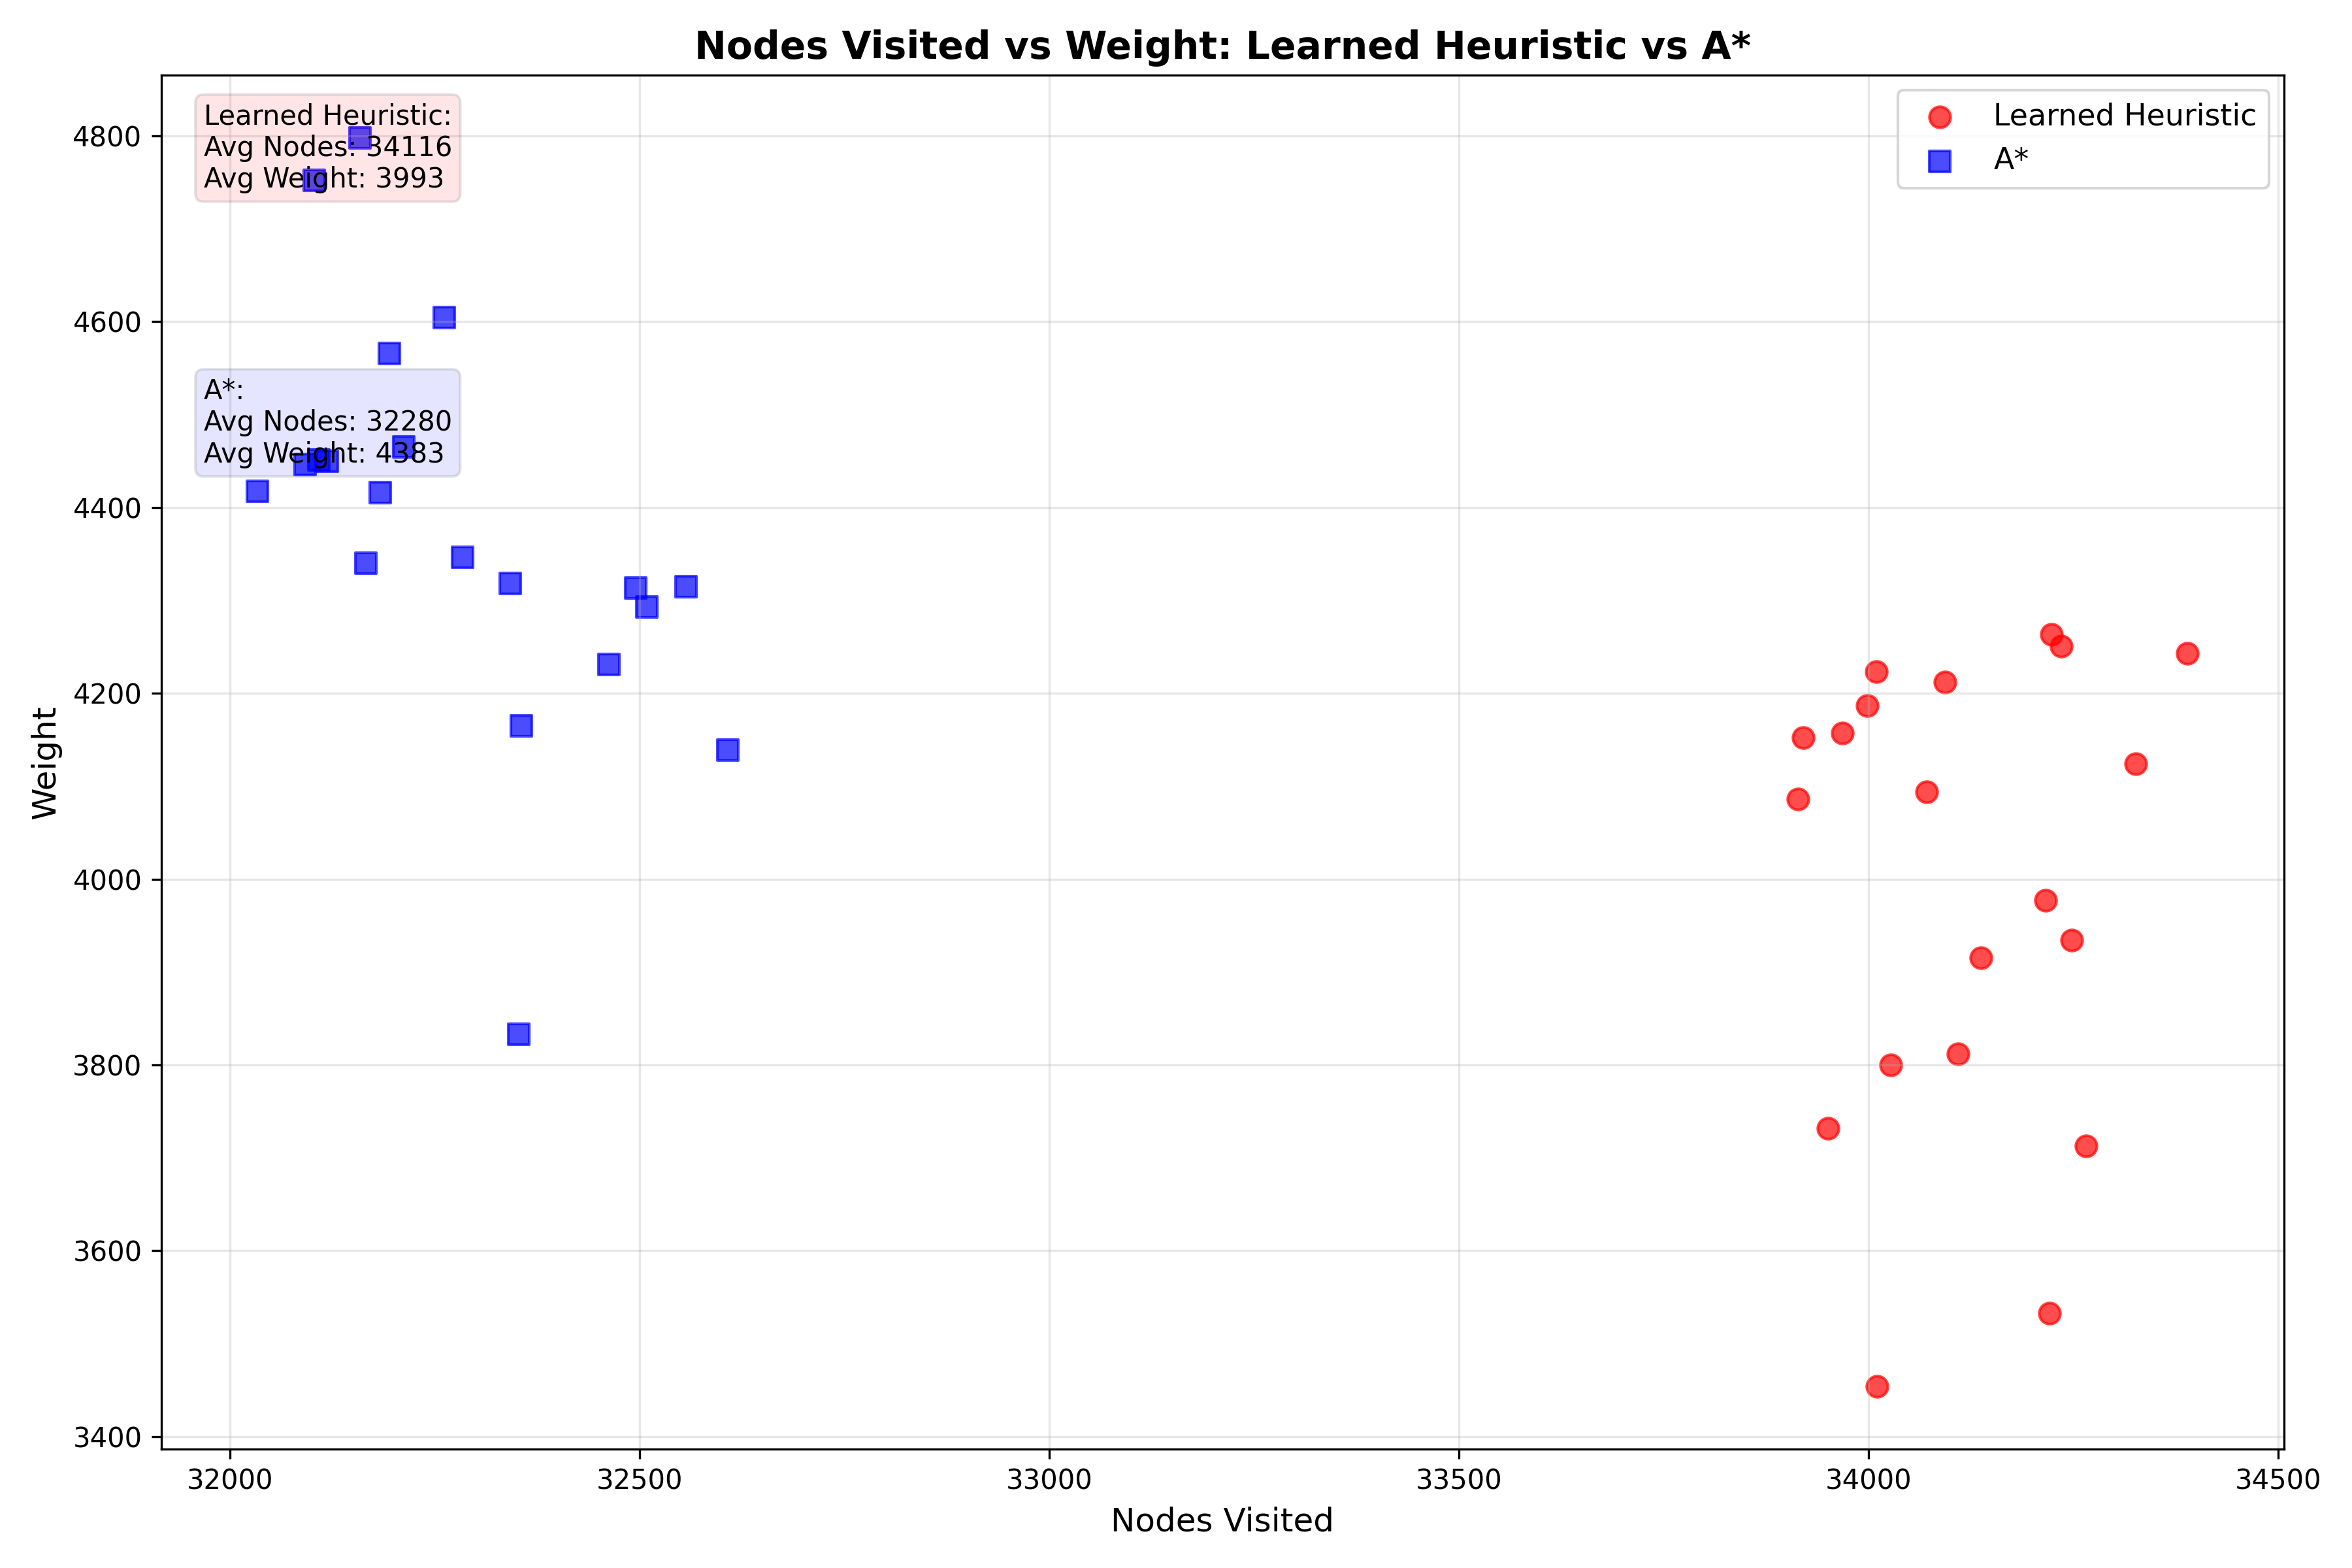
\includegraphics[width=0.7\textwidth]{../nodes_vs_weight_comparison.png}
  \end{center}

  Jak widać na zamieszczonym wykresie, wytrenowana heurystyka odwiedza więcej
  węzłów niż A*, ale jest w stanie znaleźć rozwiązanie z mniejszą sumą wag.

  Poniżej znajduje się parę ciekawszych przykładów rozbieżności A* i wytrenowanej heurystyki:

  \begin{center}
    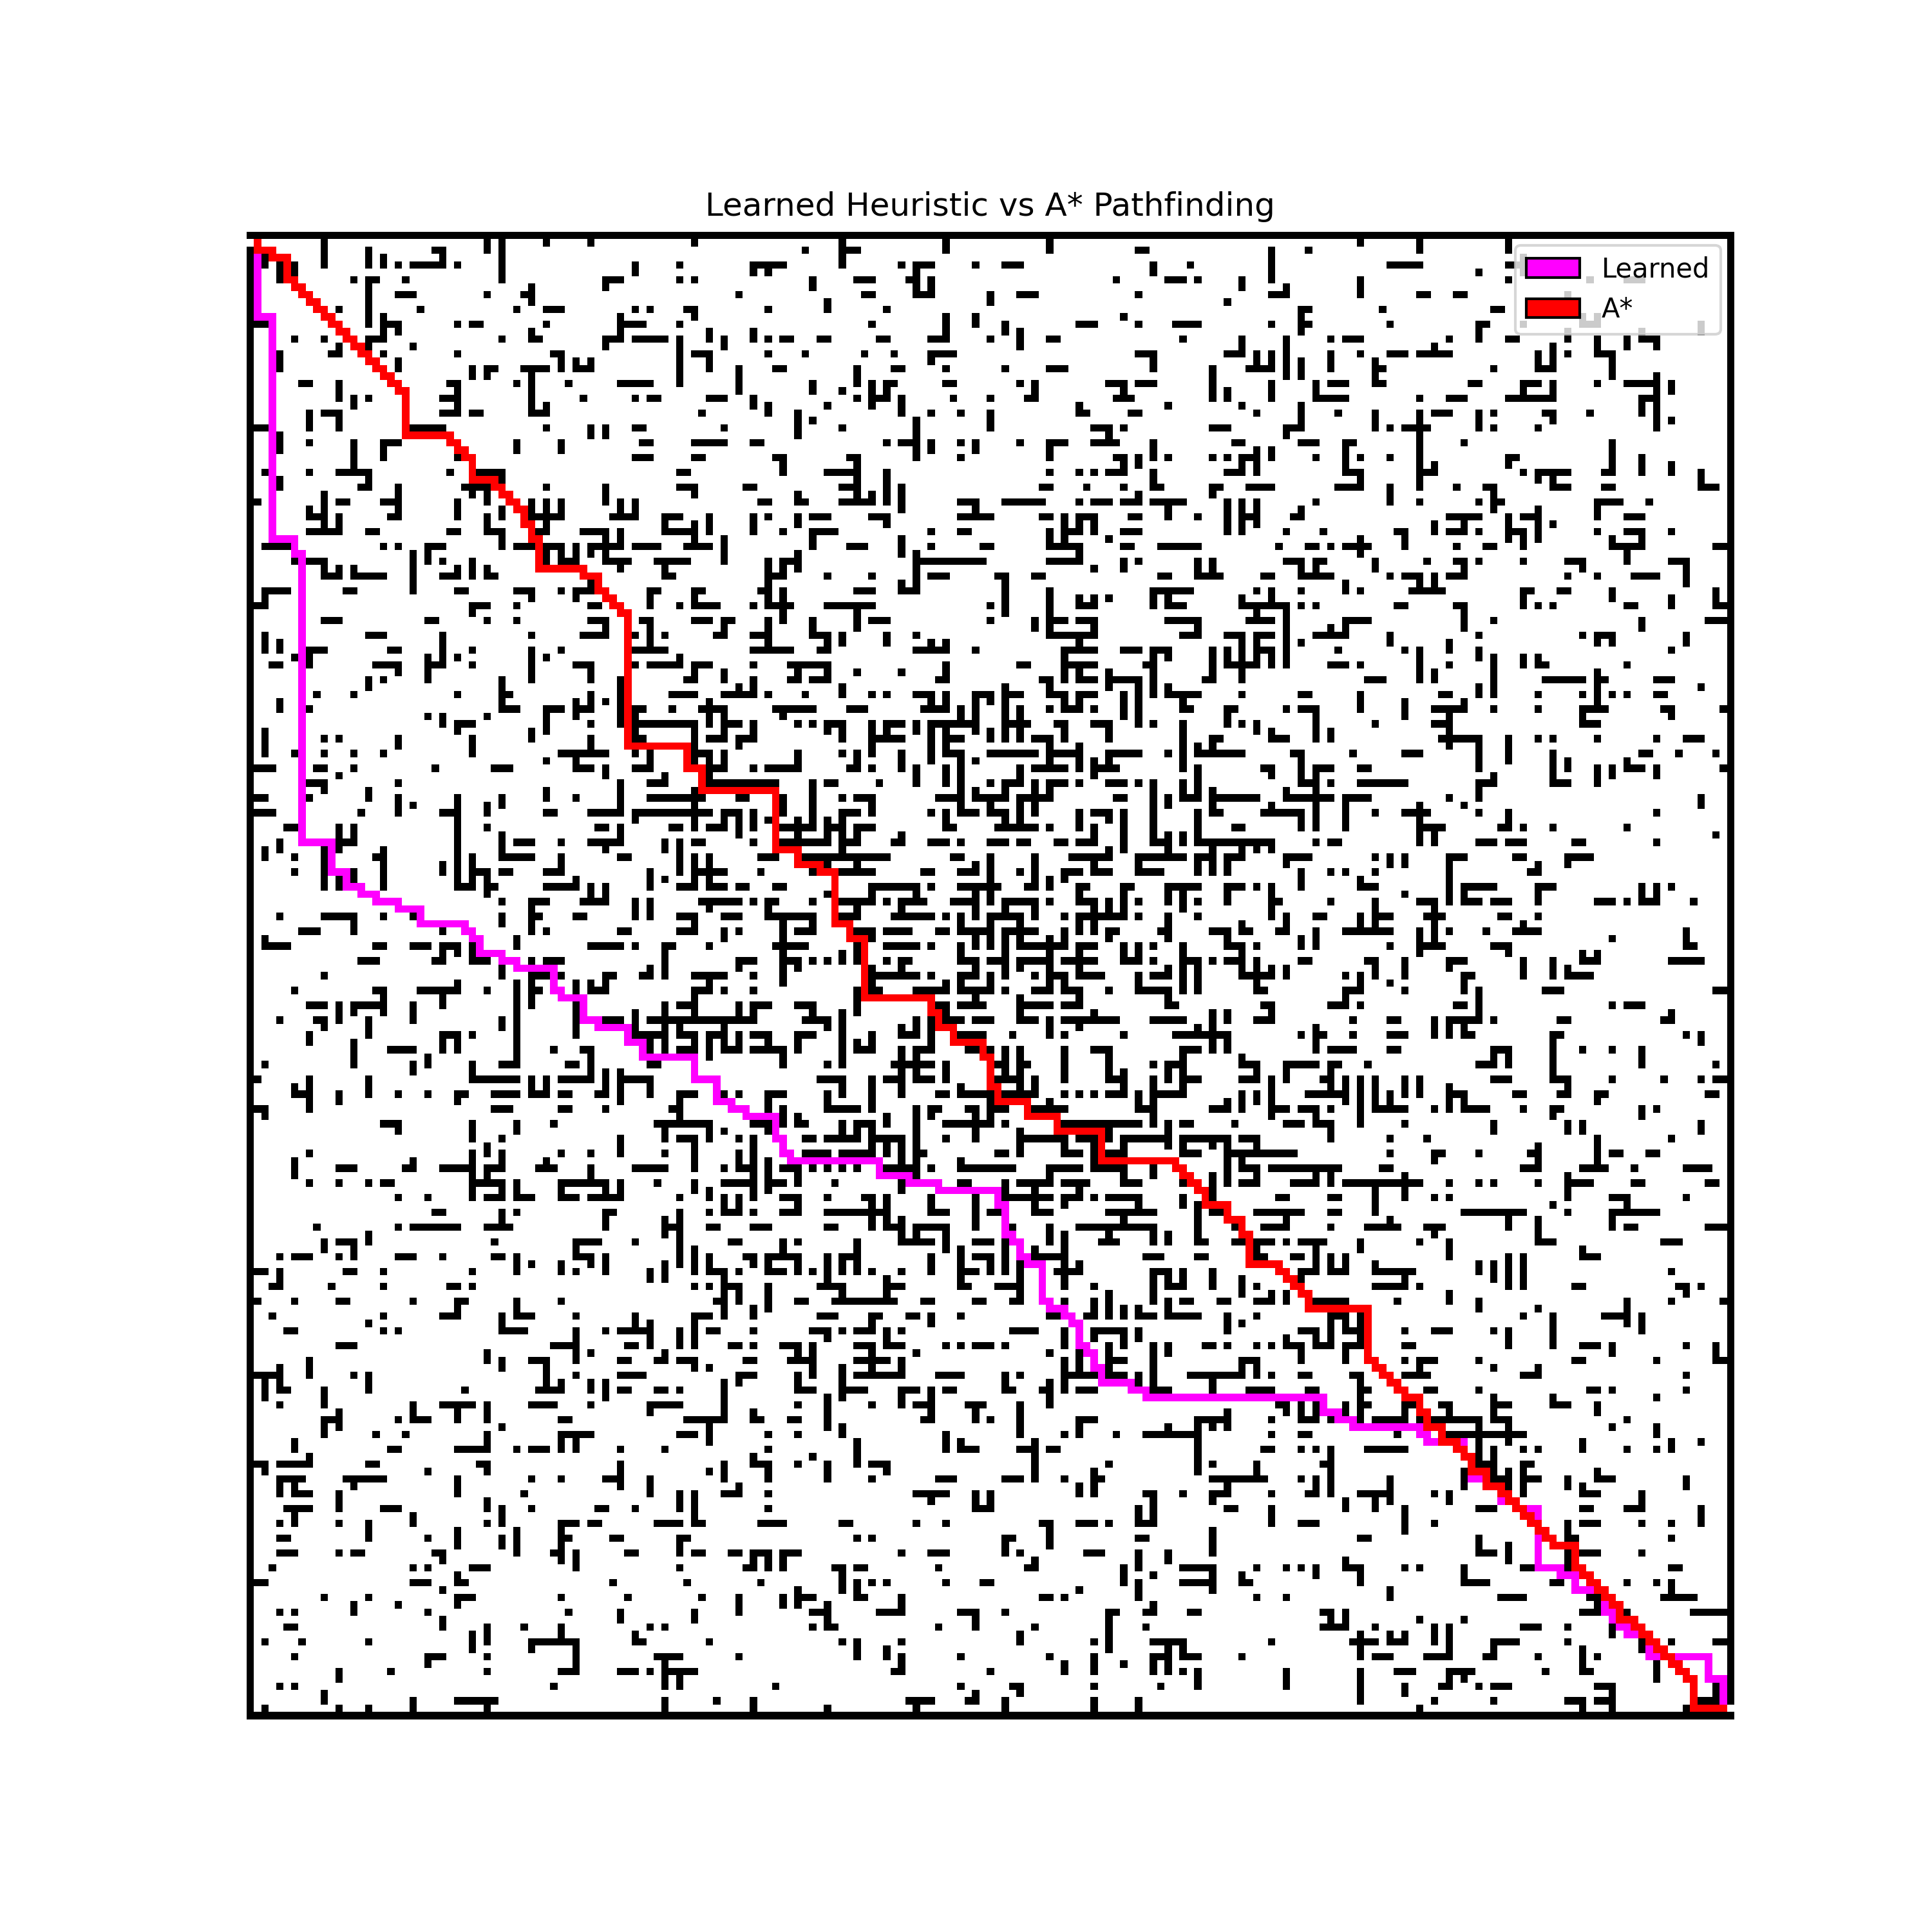
\includegraphics[width=0.7\textwidth]{../images/interesting_case1.png}
  \end{center}
  \begin{center}
    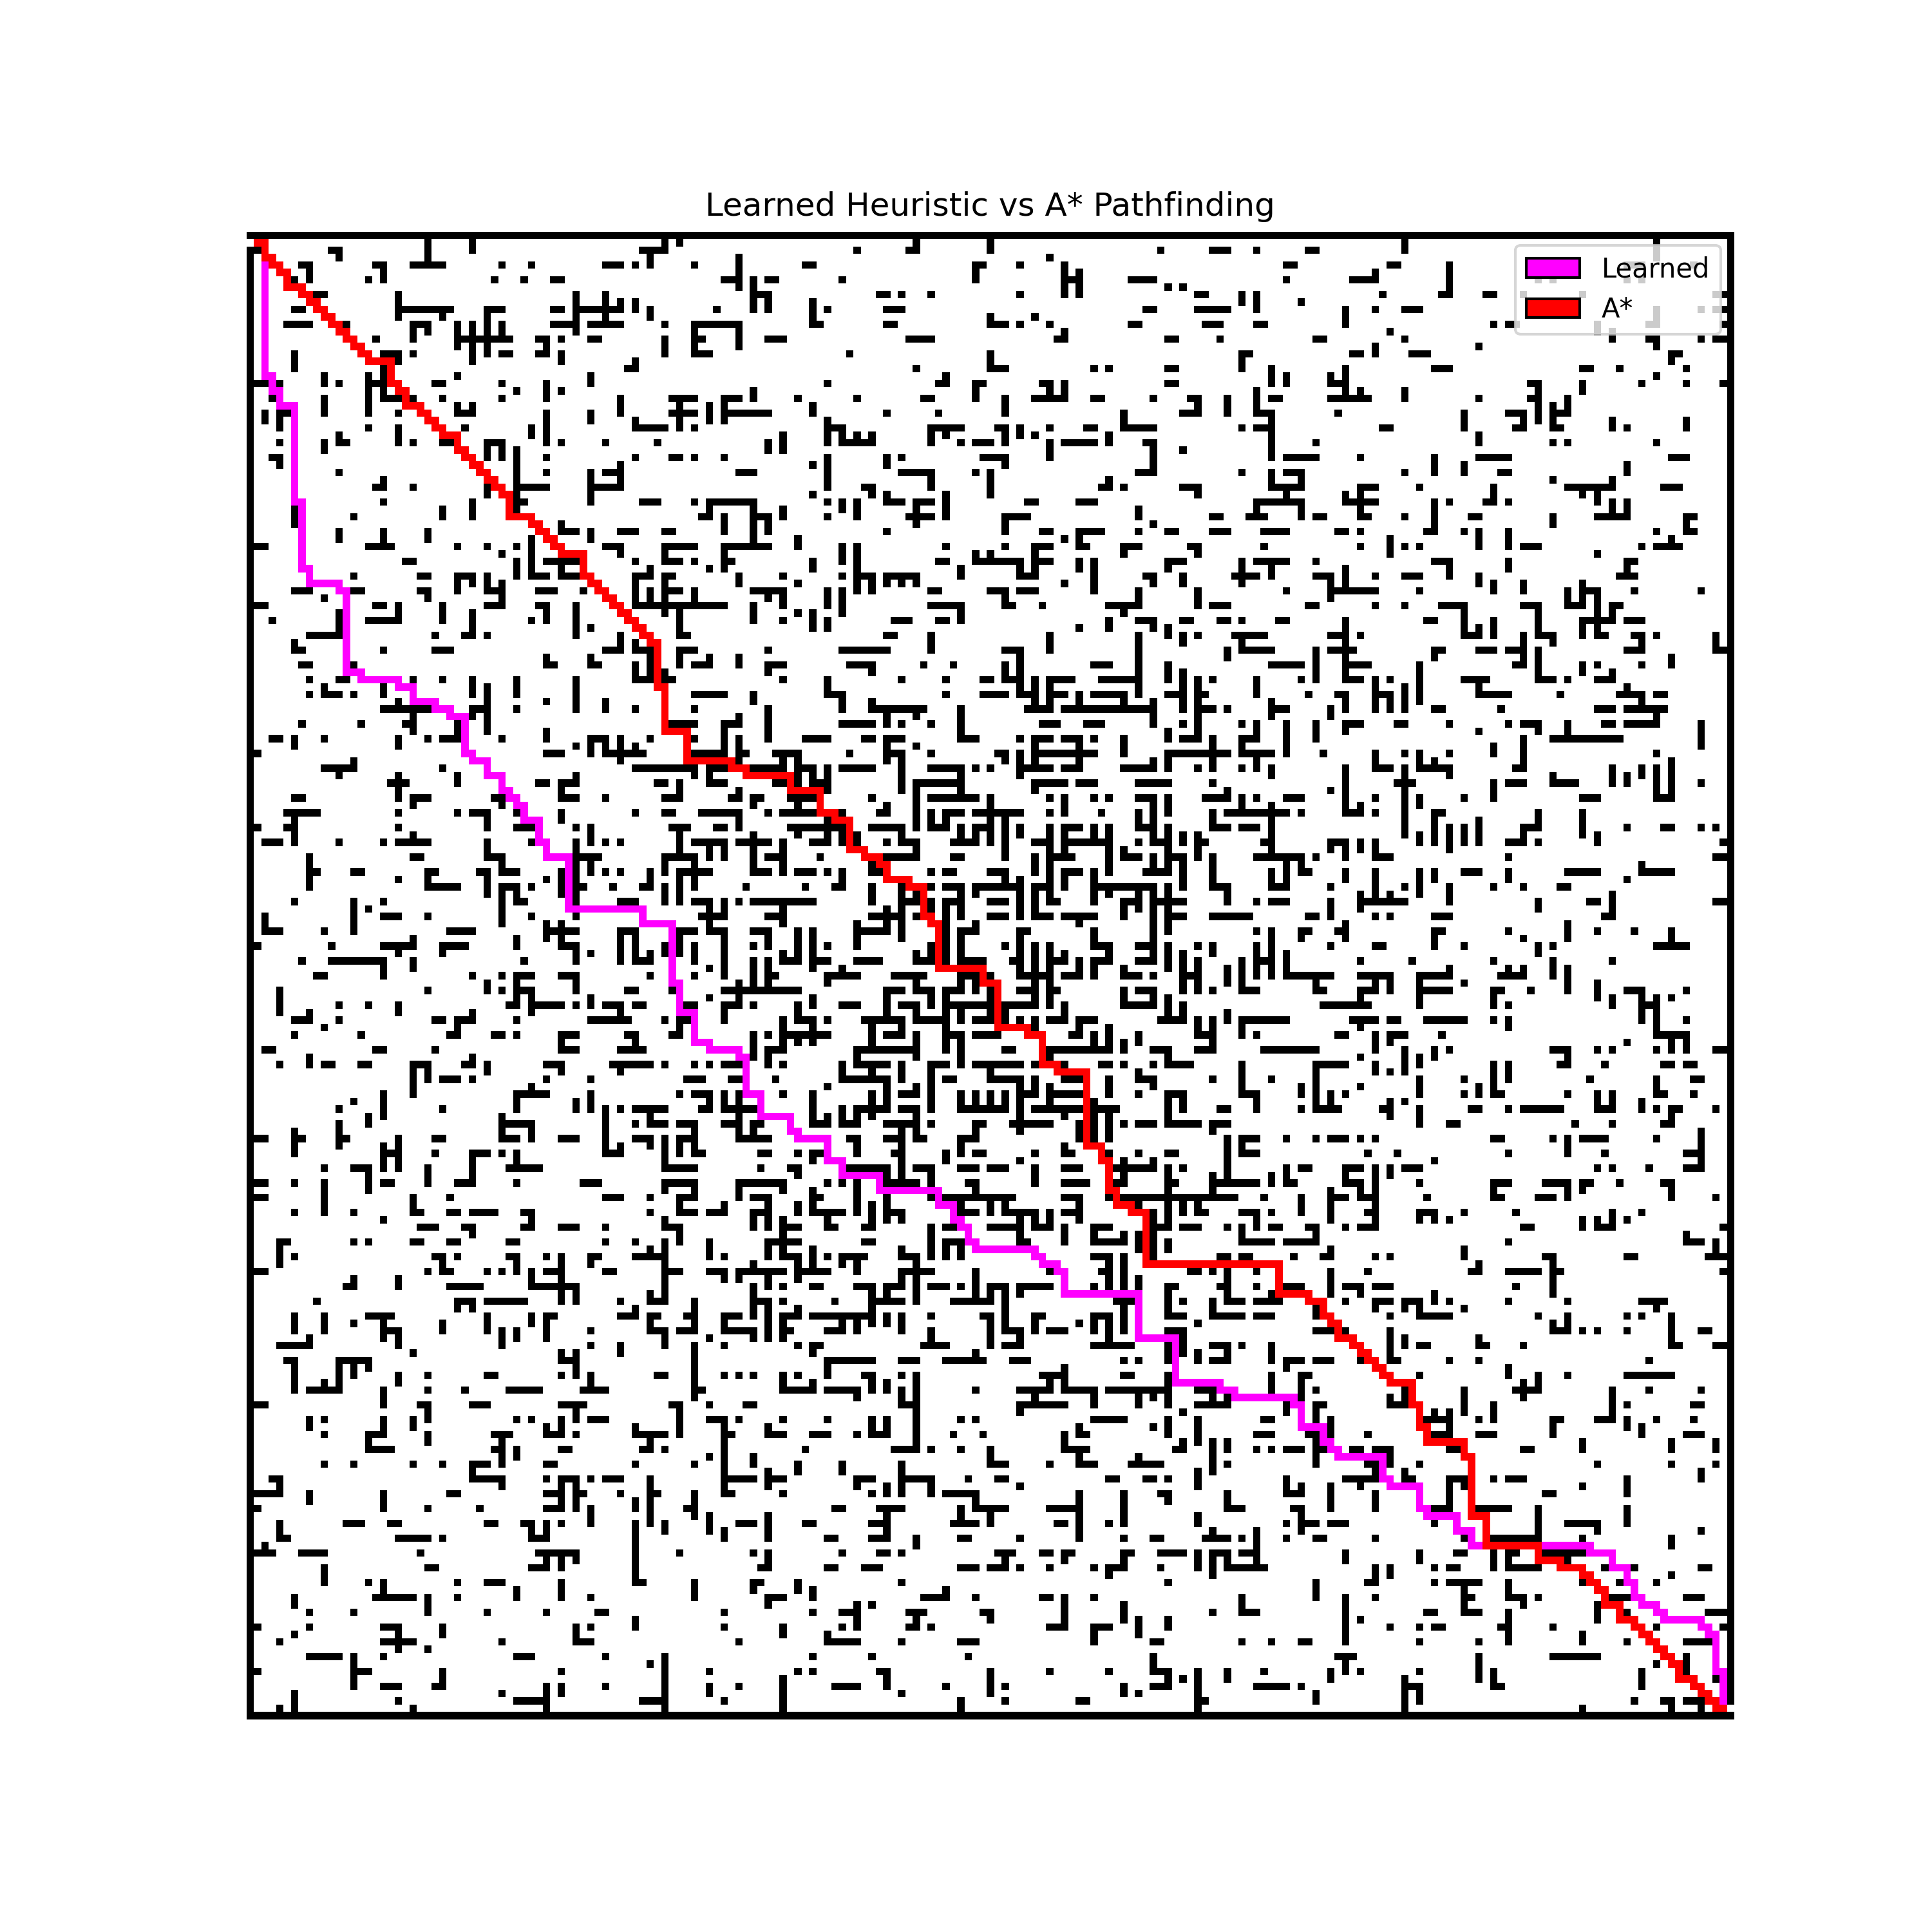
\includegraphics[width=0.7\textwidth]{../images/interesting_case2.png}
  \end{center}

  \subsection{Wnioski}
  Wytrenowana heurystyka znajduje rozwiązania z mniejszą sumą wag niż A*,
  lecz odwiedza więcej węzłów. Niestety trenowanie modelu jest bardzo niewydajne
  obliczeniowo, tak jak i wyciąganie z niego heurystyki. Skalowanie wyuczonej
  heurystyki na większe labirynty jest znacznym plusem dla tego rozwiązania,
  lecz wyuczenie modelu jest czasochłonne i musiałoby być przeprowadzane dla
  każdego rozłożenia gęstości ścian w labiryncie osobno.

  \section{Narzędzia pomocnicze}
  Projekt nie byłby możliwy bez użycia kilku narzędzi, które znacznie
  ułatwiły pracę. Do generowania labiryntów użyliśmy algorytmu Kruskala,
  natomiast do generowania tablicy wag użyliśmy konwolucji z jądrem
  zaimplementowanej w bibliotece Scipy.

\end{document}
